\documentclass[12pt,a4paper]{article}
\usepackage[utf8]{inputenc}
\usepackage[T1]{fontenc}
\usepackage[brazilian]{babel}
\usepackage{amsmath,amssymb}
\usepackage{graphicx}
\usepackage{booktabs}
\usepackage{listings}
\usepackage{xcolor}
\usepackage{hyperref}
\usepackage[margin=2.5cm]{geometry}
\usepackage{fancyhdr}
\usepackage{float}
\usepackage{lmodern}

% Estilo de código
\lstset{
    basicstyle=\ttfamily\small,
    breaklines=true,
    frame=single,
    backgroundcolor=\color{gray!5},
    keywordstyle=\color{blue!70!black},
    commentstyle=\color{green!50!black},
    stringstyle=\color{red!60!black},
    numbers=left,
    numberstyle=\tiny\color{gray},
    language=C,
    tabsize=4,
    showstringspaces=false,
    extendedchars=true,
    literate={á}{{\'a}}1 {é}{{\'e}}1 {í}{{\'i}}1 {ó}{{\'o}}1 {ú}{{\'u}}1
             {Á}{{\'A}}1 {É}{{\'E}}1 {Í}{{\'I}}1 {Ó}{{\'O}}1 {Ú}{{\'U}}1
             {à}{{\`a}}1 {è}{{\`e}}1 {ì}{{\`i}}1 {ò}{{\`o}}1 {ù}{{\`u}}1
             {À}{{\`A}}1 {È}{{\'E}}1 {Ì}{{\`I}}1 {Ò}{{\`O}}1 {Ù}{{\`U}}1
             {ã}{{\~a}}1 {ẽ}{{\~e}}1 {ĩ}{{\~i}}1 {õ}{{\~o}}1 {ũ}{{\~u}}1
             {Ã}{{\~A}}1 {Ẽ}{{\~E}}1 {Ĩ}{{\~I}}1 {Õ}{{\~O}}1 {Ũ}{{\~U}}1
             {â}{{\^a}}1 {ê}{{\^e}}1 {î}{{\^i}}1 {ô}{{\^o}}1 {û}{{\^u}}1
             {Â}{{\^A}}1 {Ê}{{\^E}}1 {Î}{{\^I}}1 {Ô}{{\^O}}1 {Û}{{\^U}}1
             {ç}{{\c c}}1 {Ç}{{\c C}}1,
}

\pagestyle{fancy}
\fancyhf{}
\rhead{Hugo Leandro Antunes — 123143543}
\lhead{Trabalho 1 — MPI}
\rfoot{\thepage}

\begin{document}

% ===================================================================
% CAPA
% ===================================================================
\begin{titlepage}
    \centering
    \vspace*{3cm}
    {\Huge\bfseries Trabalho 1 — MPI\\[0.5cm]}
    {\Large Computação de Alto Desempenho}\\[2cm]
    {\Large Hugo Leandro Antunes}\\[0.5cm]
    {\large DRE: 123143543}\\[2cm]
    {\large \today}
    \vfill
\end{titlepage}

\tableofcontents
\newpage

% ===================================================================
% EXERCÍCIO 1
% ===================================================================
\section{Exercício 1 — Variantes do Hello World}

\subsection{Exercício 1(a) — Introspecção em nível de SO}

\textbf{Abordagem:} Cada processo MPI reporta, além do seu rank e número total de
processos, o PID do processo no sistema operacional (via \texttt{getpid()}) e o
núcleo de CPU em que está executando (via \texttt{sched\_getcpu()}).

\textbf{Compilação e execução:}
\begin{lstlisting}[language=bash,numbers=none]
mpicc -O2 -Wall -o hello_os hello_os.c
mpiexec -n 8 ./hello_os
\end{lstlisting}

\textbf{Saída de 3 execuções consecutivas:}

\begin{lstlisting}[language={},numbers=none]
>> Execução 1:
Hello from rank 0/8 -- PID = 739, CPU = 10
...
Hello from rank 7/8 -- PID = 755, CPU = 6

>> Execução 2:
Hello from rank 0/8 -- PID = 766, CPU = 14
...
Hello from rank 7/8 -- PID = 783, CPU = 10

... (execuções 3 a 19 omitidas por brevidade) ...

>> Execução 20:
Hello from rank 0/8 -- PID = 904, CPU = 8
Hello from rank 1/8 -- PID = 905, CPU = 4
Hello from rank 2/8 -- PID = 906, CPU = 11
Hello from rank 3/8 -- PID = 910, CPU = 3
Hello from rank 4/8 -- PID = 912, CPU = 0
Hello from rank 5/8 -- PID = 915, CPU = 14
Hello from rank 6/8 -- PID = 919, CPU = 6
Hello from rank 7/8 -- PID = 921, CPU = 7
\end{lstlisting}

\textbf{Observações:}
\begin{enumerate}
    \item \textbf{PIDs distintos:} Em cada execução, todos os 8 ranks possuem PIDs
    diferentes, confirmando que cada rank é um processo real do SO que roda
    concorrentemente.
    \item \textbf{CPUs variando:} A coluna de CPU muda entre execuções. Isso ocorre
    porque o escalonador do kernel do Linux decide em qual núcleo cada processo é
    executado, e essa decisão é não-determinística — depende da carga do sistema
    no momento.
\end{enumerate}

\subsection{Exercício 1(b) — Variante em anel}

\textbf{Abordagem:} Cada rank $k$ envia sua saudação ao rank $(k+1) \bmod p$ e recebe
do rank $(k-1+p) \bmod p$, formando um anel.

\textbf{Escolha de implementação — \texttt{MPI\_Sendrecv}:}
Optei por \texttt{MPI\_Sendrecv} em vez de reordenar \texttt{Send}/\texttt{Recv}
manualmente. A justificativa é que \texttt{MPI\_Sendrecv} é uma operação atômica que
realiza envio e recebimento simultaneamente, eliminando completamente o risco de
deadlock circular. Um anel ingênuo com \texttt{Recv}-antes-de-\texttt{Send} gera
deadlock porque todos os ranks ficam bloqueados esperando receber do vizinho à
esquerda antes de enviar ao vizinho à direita.

O operador $+\,p$ em $(k - 1 + p) \bmod p$ garante argumento não-negativo para
\texttt{\%} em C, que retorna o sinal do dividendo.

\textbf{Compilação e execução:}
\begin{lstlisting}[language=bash,numbers=none]
mpicc -O2 -Wall -o hello_ring hello_ring.c
mpiexec -n 4 ./hello_ring
\end{lstlisting}

\textbf{Saída:}
\begin{lstlisting}[language={},numbers=none]
Rank 0 received from Rank 3: 'Greetings from rank 3 of 4!'
Rank 1 received from Rank 0: 'Greetings from rank 0 of 4!'
Rank 2 received from Rank 1: 'Greetings from rank 1 of 4!'
Rank 3 received from Rank 2: 'Greetings from rank 2 of 4!'
\end{lstlisting}

% ===================================================================
% EXERCÍCIO 2
% ===================================================================
\section{Exercício 2 — Regra do Trapézio Generalizada}

\textbf{Compilação e execução (geral para as variantes do Exercício 2):}
\begin{lstlisting}[language=bash,numbers=none]
mpicc -O2 -Wall -o mpi_trap_generalized mpi_trap_generalized.c -lm
mpiexec -n 3 ./mpi_trap_generalized 0 3.14159265358979323846 10
\end{lstlisting}

\subsection{Exercício 2(a) — Balanceamento de carga para $n$ arbitrário}

\textbf{Abordagem:} Parti do código \texttt{mpi\_trap\_input.c} da aula e
substituí a divisão uniforme $\texttt{local\_n} = n / p$ pelo esquema com resto:

\begin{lstlisting}[language=C]
int rem      = n % comm_sz;
int local_n  = n / comm_sz + (my_rank < rem ? 1 : 0);
int offset   = my_rank * (n / comm_sz)
             + (my_rank < rem ? my_rank : rem);
double local_a = a + offset * h;
double local_b = local_a + local_n * h;
\end{lstlisting}

Os primeiros $n \bmod p$ ranks recebem $\lceil n/p \rceil$ trapézios, e os demais
recebem $\lfloor n/p \rfloor$. A função de integração é $f(x) = \sin(x)$.

\textbf{Verificação com $p = 3$, $n = 10$, $\int_0^\pi \sin(x)\,dx = 2$:}

Divisão: $10 \bmod 3 = 1$, então rank 0 fica com 4 trapézios, ranks 1 e 2 com 3 cada.

\begin{lstlisting}[language={},numbers=none]
RESULT: p=3 n=10 integral=1.983523537509454e+00 Tp=0.000011
  Exact = 2.000000000000000e+00, Error = 1.6476e-02, h = 3.1416e-01
\end{lstlisting}

\subsection{Exercício 2(b) — Estudo de escalabilidade forte}

\textbf{Definição:} $T_s$ é o tempo de relógio do código MPI executado com $p = 1$
(inclui overhead de \texttt{MPI\_Init}/\texttt{MPI\_Finalize}).
Fixei $n = 10^7$ e tabulei para $p \in \{1, 2, 4, 8\}$. Cada configuração foi
executada 11 vezes e o valor reportado é a \textbf{mediana}, eliminando outliers
causados por variações do escalonador do SO.

\begin{table}[H]
    \centering
    \caption{Escalabilidade forte — $n = 10^7$, $f(x) = \sin(x)$ em $[0, \pi]$ (mediana de 11 execuções).}
    \begin{tabular}{@{}rrrr@{}}
        \toprule
        $p$ & $T_p$ (s) & $S_p = T_1/T_p$ & $E_p = S_p/p$ \\
        \midrule
        1 & 0.065372 & 1.0000 & 1.0000 \\
        2 & 0.034137 & 1.9150 & 0.9575 \\
        4 & 0.017820 & 3.6685 & 0.9171 \\
        8 & 0.011797 & 5.5414 & 0.6927 \\
        \bottomrule
    \end{tabular}
    \label{tab:scalability}
\end{table}

\begin{figure}[H]
    \centering
    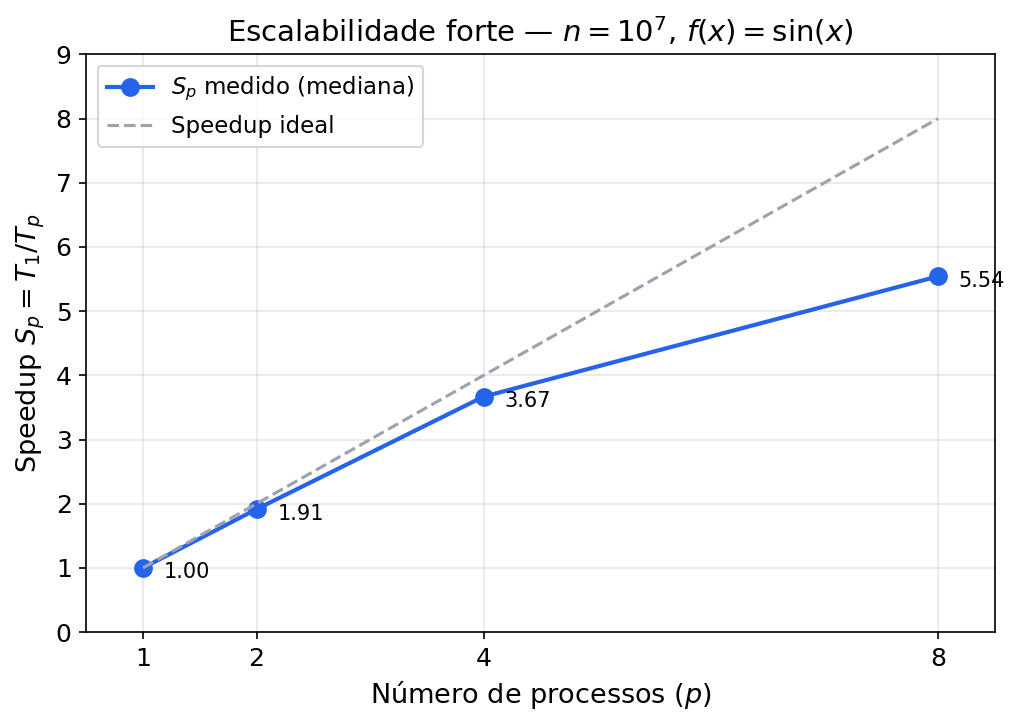
\includegraphics[width=0.8\textwidth]{results/scalability_speedup.png}
    \caption{Speedup $S_p$ vs.\ número de processos $p$ (escalabilidade forte, $n = 10^7$).}
    \label{fig:speedup}
\end{figure}

\begin{figure}[H]
    \centering
    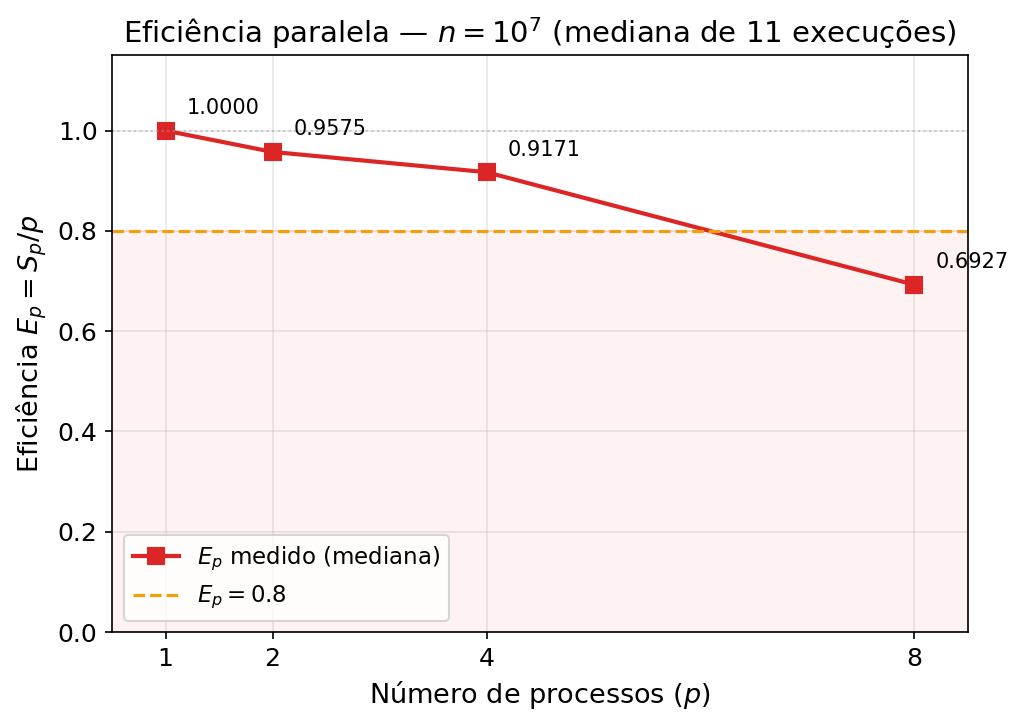
\includegraphics[width=0.8\textwidth]{results/scalability_efficiency.png}
    \caption{Eficiência $E_p$ vs.\ número de processos $p$ ($n = 10^7$, mediana de 11 execuções).}
    \label{fig:efficiency}
\end{figure}

\textbf{Discussão:} A eficiência $E_p$ permanece acima de 0.9 para $p \leq 4$,
mas cai para $\approx 0.69$ em $p = 8$. A máquina de teste possui 8 núcleos
físicos (AMD Ryzen 7 8700G), portanto não há oversubscription em $p = 8$.
A queda de eficiência se explica pela granularidade fina do trabalho: com
$n/p = 1{,}25 \times 10^6$ trapézios por processo e tempo total $\sim 12$~ms,
a latência fixa de comunicação (\texttt{MPI\_Reduce}) e sincronização
(\texttt{MPI\_Barrier}) domina proporcionalmente mais o tempo total.
A eficiência cai abaixo de 0.8 a partir de $p = 8$.

\subsection{Exercício 2(c) — Bônus: Convergência $O(h^2)$}

Fixei $p = 4$ e variei $n \in \{64, 256, 1024, 4096, 16384\}$.

\begin{figure}[H]
    \centering
    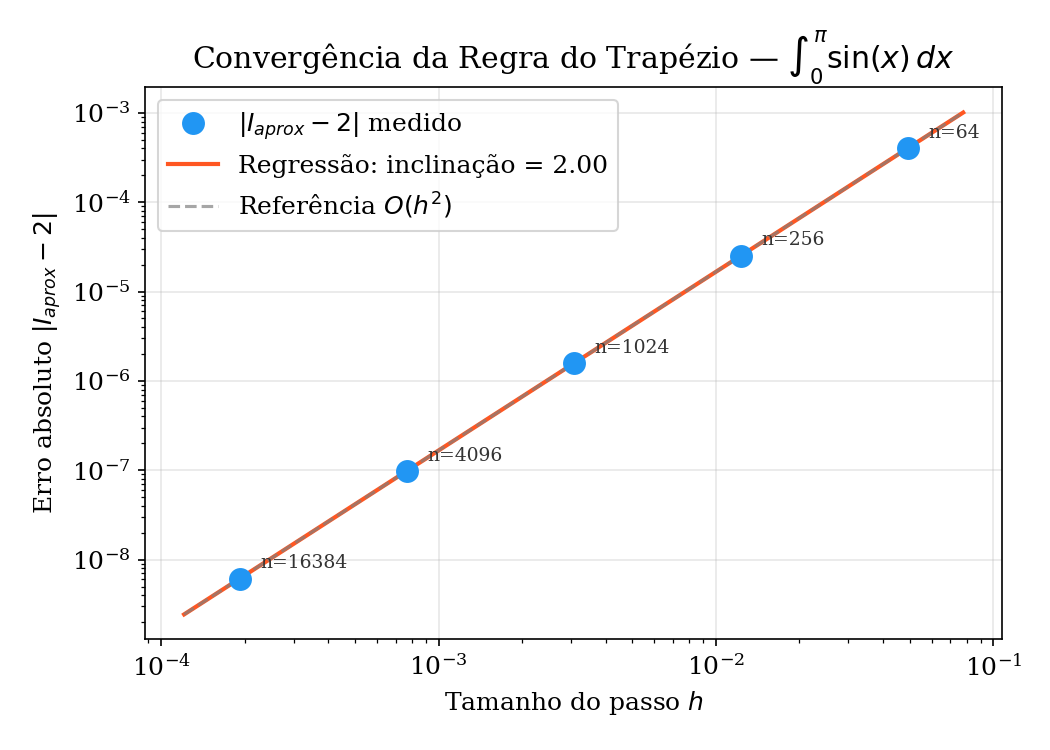
\includegraphics[width=0.8\textwidth]{results/convergence_loglog.png}
    \caption{Convergência log-log: $|\text{erro}|$ vs.\ $h$ para a regra do trapézio.}
    \label{fig:convergence}
\end{figure}

\textbf{Resultado:} A inclinação da reta de regressão em escala log-log é $\approx 2.0$,
confirmando a taxa de convergência $O(h^2)$ da regra do trapézio composta.

% ===================================================================
% EXERCÍCIO 3
% ===================================================================
\section{Exercício 3 — Soma Paralela}

\textbf{Abordagem:}
\begin{enumerate}
    \item Rank 0 gera vetor de $N = 10^7$ doubles aleatórios (seed fixa = 42).
    \item Rank 0 distribui $N/p$ elementos a cada rank via laço de \texttt{MPI\_Send}.
    \item Cada rank calcula soma local.
    \item Cada rank envia soma parcial ao rank 0 via \texttt{MPI\_Send}.
    \item Rank 0 soma as parciais e compara com soma serial.
\end{enumerate}

\textbf{Compilação e execução:}
\begin{lstlisting}[language=bash,numbers=none]
mpicc -O2 -Wall -o mpi_psum mpi_psum.c -lm
mpiexec -n 4 ./mpi_psum 10000000
\end{lstlisting}

\textbf{Saída:}
\begin{lstlisting}[language={},numbers=none]
N = 10000000, p = 4
Soma serial   = 4.999361300896658e+06
Soma paralela = 4.999361300896985e+06
Erro relativo = 6.5573e-14
\end{lstlisting}

\textbf{Análise:} O erro relativo é da ordem de $10^{-14}$, decorrente da
reordenação de ponto flutuante — a ordem das somas parciais difere entre as
versões serial e paralela, e o acúmulo de erros de arredondamento ao longo de
$N = 10^7$ operações amplifica a diferença para além da precisão de máquina
unitária ($\varepsilon \approx 10^{-16}$).

\textbf{Comparação com versão coletiva (Aula 6):}
Na versão com coletivas, o pipeline \texttt{MPI\_Send} + \texttt{MPI\_Recv}
é substituído por \texttt{MPI\_Scatter} (distribuição) e \texttt{MPI\_Reduce}
(redução). Isso reduz significativamente a quantidade de código:

\begin{table}[H]
    \centering
    \caption{Comparação de linhas de código — soma paralela.}
    \begin{tabular}{@{}lr@{}}
        \toprule
        Versão & Linhas de código \\
        \midrule
        Ponto-a-ponto (\texttt{Send/Recv}) & $\sim$90 \\
        Coletivas (\texttt{Scatter/Reduce}) & $\sim$40 \\
        \bottomrule
    \end{tabular}
\end{table}

% ===================================================================
% EXERCÍCIO 4
% ===================================================================
\section{Exercício 4 — Prática de Comunicação Coletiva}

\subsection{Exercício 4(a) — Hello com \texttt{MPI\_Gather}}

\textbf{Abordagem:} Cada rank prepara uma saudação em um buffer de tamanho fixo
(\texttt{MAX\_STRING = 100}). O rank 0 usa \texttt{MPI\_Gather} para coletar
todas as saudações em um vetor contíguo, substituindo o laço de \texttt{MPI\_Recv}
do código original.

\textbf{Compilação e execução:}
\begin{lstlisting}[language=bash,numbers=none]
mpicc -O2 -Wall -o hello_gather hello_gather.c
mpiexec -n 4 ./hello_gather
\end{lstlisting}

\textbf{Saída:}
\begin{lstlisting}[language={},numbers=none]
Greetings from process 0 of 4!
Greetings from process 1 of 4!
Greetings from process 2 of 4!
Greetings from process 3 of 4!
\end{lstlisting}

\subsection{Exercício 4(b) — Máx/mín global com \texttt{MPI\_Reduce}}

\textbf{Abordagem:} Rank 0 gera $N = 10^6$ doubles aleatórios em $[-500, 500]$.
\texttt{MPI\_Scatter} distribui blocos iguais. Cada rank calcula máx e mín locais.
\texttt{MPI\_Reduce} com \texttt{MPI\_MAX} e \texttt{MPI\_MIN} produz os extremos
globais. Rank 0 verifica contra percurso serial.

\textbf{Compilação e execução:}
\begin{lstlisting}[language=bash,numbers=none]
mpicc -O2 -Wall -o minmax minmax.c -lm
mpiexec -n 4 ./minmax 1000000
\end{lstlisting}

\textbf{Saída:}
\begin{lstlisting}[language={},numbers=none]
N = 1000000, p = 4
MPI_Reduce  MAX = 499.999,  MIN = -499.998
Serial      MAX = 499.999,  MIN = -499.998
Verificação: MAX OK, MIN OK
\end{lstlisting}

% ===================================================================
% EXERCÍCIO 5
% ===================================================================
\section{Exercício 5 — Soma Paralela de Vetores}

\textbf{Abordagem:} Rank 0 inicializa $x_i = i$ e $y_i = 2i$.
\texttt{MPI\_Scatter} distribui blocos de $x$ e $y$. Cada rank computa
$z_{\text{local}} = x_{\text{local}} + y_{\text{local}}$.

\textbf{Compilação e execução:}
\begin{lstlisting}[language=bash,numbers=none]
mpicc -O2 -Wall -o mpi_vecadd_gather mpi_vecadd_gather.c
mpiexec -n 4 ./mpi_vecadd_gather 16

mpicc -O2 -Wall -o mpi_vecadd_allgather mpi_vecadd_allgather.c
mpiexec -n 4 ./mpi_vecadd_allgather 16
\end{lstlisting}

\subsection{Versão com \texttt{MPI\_Gather}}
Rank 0 coleta $z$ via \texttt{MPI\_Gather} e verifica $z_i = 3i$.

\subsection{Versão com \texttt{MPI\_Allgather}}
Todos os ranks recebem o vetor $z$ completo via \texttt{MPI\_Allgather}.
Cada rank verifica localmente.

\textbf{Saídas:}
\begin{lstlisting}[language={},numbers=none]
=== Gather ===
z = x + y (Gather):
  z[ 0] = 0  (expected 0)
  z[ 1] = 3  (expected 3)
...
  z[15] = 45  (expected 45)
Verificação: OK

=== Allgather ===
[Rank 0] z = x + y (Allgather):
  z[ 0] = 0
...
  z[15] = 45
  Verificação: OK
[Rank 1] z = x + y (Allgather): ...
[Rank 2] z = x + y (Allgather): ...
[Rank 3] z = x + y (Allgather): ...
\end{lstlisting}

\textbf{Discussão — Quando \texttt{MPI\_Allgather} é preferível:}

\texttt{MPI\_Allgather} é útil quando \textit{todos} os processos precisam do
resultado completo para computação subsequente. Exemplos:
\begin{itemize}
    \item \textbf{Multiplicação matriz-vetor iterativa:} Em métodos como Gradiente
    Conjugado, cada rank calcula uma parte de $y = Ax$, mas todos precisam do vetor
    $y$ completo para a próxima iteração.
    \item \textbf{Busca global:} Quando cada processo precisa saber o estado global
    para tomar decisões locais (ex: critérios de convergência).
\end{itemize}

A desvantagem é o custo de comunicação: \texttt{MPI\_Allgather} envia $O(N)$ dados
a \textit{todos} os ranks, enquanto \texttt{MPI\_Gather} envia apenas ao root.

% ===================================================================
% EXERCÍCIO 6
% ===================================================================
\section{Exercício 6 — Tipo de Dado Derivado MPI}

\textbf{Struct:}
\begin{lstlisting}[language=C]
struct Student {
    char   name[50];
    double grade;
    int    id;
};
\end{lstlisting}

\textbf{Compilação e execução:}
\begin{lstlisting}[language=bash,numbers=none]
mpicc -O2 -Wall -o student_struct student_struct.c
mpiexec -n 4 ./student_struct

mpicc -O2 -Wall -o student_three_bcasts student_three_bcasts.c
mpiexec -n 4 ./student_three_bcasts
\end{lstlisting}

\subsection{Versão com tipo derivado}
Construí um tipo MPI com \texttt{MPI\_Type\_create\_struct} usando
\texttt{offsetof} de \texttt{<stddef.h>} para deslocamentos corretos
(que respeitam o padding inserido pelo compilador).
Uma única chamada \texttt{MPI\_Bcast} transmite o registro completo.

\subsection{Versão com três \texttt{MPI\_Bcast}}
Três chamadas separadas: uma para \texttt{name} (50 chars), uma para
\texttt{grade} (1 double), uma para \texttt{id} (1 int).

\textbf{Comparação:}
\begin{table}[H]
    \centering
    \caption{Comparação entre tipo derivado e três Bcasts.}
    \begin{tabular}{@{}lcc@{}}
        \toprule
        Versão & Chamadas MPI\_Bcast & Conteúdo idêntico? \\
        \midrule
        Tipo derivado & 1 & Sim \\
        Três Bcasts   & 3 & Sim \\
        \bottomrule
    \end{tabular}
\end{table}

O conteúdo recebido é \textbf{idêntico} em ambas versões. A vantagem do tipo
derivado é:
\begin{enumerate}
    \item \textbf{Eficiência:} Menos chamadas MPI reduz latência acumulada
    (cada \texttt{Bcast} incorre em overhead de sincronização $O(\log p)$).
    \item \textbf{Escalabilidade:} Para structs com muitos campos, o número de
    chamadas com a abordagem de Bcasts separados cresce linearmente; com tipo
    derivado, permanece 1.
    \item \textbf{Manutenabilidade:} Adicionar um campo à struct requer apenas
    atualizar a definição do tipo derivado, em vez de lembrar de adicionar mais
    uma chamada \texttt{Bcast}.
\end{enumerate}

\textbf{Saídas:}
\begin{lstlisting}[language={},numbers=none]
=== Tipo derivado (1 Bcast) ===
[Rank 0] Enviando Student via tipo derivado (1 MPI_Bcast):
  name  = "Hugo Leandro Antunes"
  grade = 9.5
  id    = 123143543
[Rank 1] Recebido via tipo derivado:
  name  = "Hugo Leandro Antunes"
  grade = 9.5
  id    = 123143543
[Rank 2] Recebido via tipo derivado:
  name  = "Hugo Leandro Antunes"
  grade = 9.5
  id    = 123143543
[Rank 3] Recebido via tipo derivado:
  name  = "Hugo Leandro Antunes"
  grade = 9.5
  id    = 123143543

=== Tres Bcasts separados ===
[Rank 0] Enviando Student via 3 MPI_Bcast separados:
  name  = "Hugo Leandro Antunes"
  grade = 9.5
  id    = 123143543
[Rank 1] Recebido via 3 Bcasts:
  name  = "Hugo Leandro Antunes"
  grade = 9.5
  id    = 123143543
[Rank 2] Recebido via 3 Bcasts:
  name  = "Hugo Leandro Antunes"
  grade = 9.5
  id    = 123143543
[Rank 3] Recebido via 3 Bcasts:
  name  = "Hugo Leandro Antunes"
  grade = 9.5
  id    = 123143543
\end{lstlisting}

\end{document}
